\documentclass[12pt]{article}

\usepackage{hcmus-report-template}

% Disable indentation on new paragraphs
\setlength{\parindent}{0pt}

% Line spacing 1.5
\renewcommand{\baselinestretch}{1.5}

% Optional: graphic path
% \graphicspath{PATH_TO_GRAPHIC_FOLDER}

% To use Times font family, uncomment this row
% \usepackage{mathptmx}

% To use roman section / subsection, uncomment these rows
% \renewcommand{\thesection}{\Roman{section}}
% \renewcommand{\thesubsection}{\thesection.\Roman{subsection}}

% Define course name, report name and report title.
\newcommand{\coursename}{Calculus I - MTH251}
\newcommand{\reportname}{Chapter 1-3}
\newcommand{\reporttitle}{Group Exercises}

\newcommand{\studentname}{Nguyễn Lê Trân (25125039) \\ Nguyễn Quang Hiếu (25125043) \\ Trần Như Khải (25125045) \\ Nguyễn Thái Bảo (25125051) \\ Trần Minh Khoa (25125057) \\ Nguyễn Anh Kiệt (25125074) \\ Nguyễn Đình Minh Huy (25125083) \\ Đặng Thanh Toàn (25125090)}
\newcommand{\teachername}{}

% Header
\lhead{\reporttitle}
\rhead{
University of Science - VNUHCM\\
\coursename
}

% Footer
\newcommand{\leftfooter}{\LaTeX\ by \href{https://github.com/ndmhuy}{Huy, Nguyen Dinh Minh}}
\lfoot{\leftfooter}

% ============ DOCUMENT ============
\begin{document}
\renewcommand{\proofname}{Proof}
\pagenumbering{roman}
\input{content/title.tex}
\thispagestyle{empty}

\begin{center}
    \textbf{\LARGE TASK ASSIGNMENT TABLE}
\end{center}
\vspace{0.5cm}

% Group Information Section
\noindent
\begin{tabular}{@{}ll}
    \textbf{\large Group Name:} & \large Brick Wizards \\ [0.5em]
    \textbf{\large Leader:} & Nguyễn Đình Minh Huy \\ [0.5em] 
\end{tabular}
\vspace{0.5cm}

% Assignment Table
\begin{table}[h]
    \centering
    \renewcommand{\arraystretch}{1.4} 
    \setlength{\tabcolsep}{4pt}      
    % Adjusted widths to fit problem lists
    \begin{tabular}{|c|c|l|p{5.0cm}|p{4.0cm}|}
        \hline
        \textbf{No.} & \textbf{ID} & \textbf{Full Name} & \textbf{Task Assignment} & \textbf{Cross-check Task} \\
        \hline
        1 & 25125039 & Nguyễn Lê Trân & Solve P10, P18 & Check P1, P5, P11, P16 \\
        \hline
        2 & 25125043 & Nguyễn Quang Hiếu & Solve P2, P12(a), P17 & Check P4, P10, P14, P18 \\
        \hline
        3 & 25125045 & Trần Như Khải & Solve P9, P16 & Check P2, P10, P17, P18 \\
        \hline
        4 & 25125051 & Nguyễn Thái Bảo & Solve P1, P7 & Check P5, P6, P9, P11 \\
        \hline
        5 & 25125057 & Trần Minh Khoa & \small \textbullet\ Format Validation \newline \textbullet\ Solve P5, P11 & Check P1, P4, P7, P14 \\
        \hline
        6 & 25125074 & Nguyễn Anh Kiệt & Solve P6, P15 & Check P2, P3, P7, P8 \\
        \hline
        7 & 25125083 & Nguyễn Đình Minh Huy & \small \textbullet\ Setup Project \newline \textbullet\ Distribute Work \newline \textbullet\ Solve P4, P14 \newline \textbullet\ Final Validation & Check P3, P8, P15, P18 \\
        \hline
        8 & 25125090 & Đặng Thanh Toàn & Solve P3, P8 & Check P6, P9, P15, P16 \\
        \hline
        \multicolumn{5}{|c|}{\textbf{Group Work (All Members):} P12(b, c, d), P13, P19, P20} \\
        \hline
    \end{tabular}
\end{table}

\pagebreak
\tableofcontents
\pagebreak
% \listoftables
% \pagebreak
% \listoffigures
% \pagebreak

\pagenumbering{arabic}
\setcounter{page}{1}

\section{Chapter 1: Functions and Models}
\subsection{Problem 1. Model selection from data}
A quantity $Q(t)$ is measured at different times $t$ (in hours), and the following data are recorded:

\begin{center}
\begin{tabular}{c|ccccc}

$t$ & 0 & 1 & 2 & 3 & 4 \\
\hline
$Q(t)$ & 100 & 80 & 64 & 51.2 & 40.96 \\

\end{tabular}
\end{center}

\begin{enumerate}[label=(\alph*)]
    \item By looking at ratios between successive values, decide whether a linear or an exponential model is more appropriate for this data. Explain your reasoning clearly.
    \item Assuming an exponential model $Q(t) = Q_{0}a^{t}$, determine the parameters $Q_{0}$ and $a$. Then rewrite the model in the form $Q(t) = Q_{0}e^{kt}$ and find $k$.
    \item Using your model, estimate the time $t$ when $Q(t)$ will first fall below 20. Comment on how sensitive your answer is to small changes in the data.
    \item Discuss at least two limitations of using this exponential model for very large $t$ (e.g., $t \gg 4$). In what real-world situation could such a model be reasonable, and when would it break down?
\end{enumerate}

\subsection*{Strategy}
\subsection*{Solution}
\begin{enumerate}[label=(\alph*)]
    \item \textbf{Model Selection} \\
    To determine the appropriate model, we check for constant differences (linear) or constant ratios (exponential).
    
    \textbf{Check for Linear (Differences):}
    \begin{itemize}
        \item $80 - 100 = -20$
        \item $64 - 80 = -16$
    \end{itemize}
    The differences are not constant, so it is \textbf{not linear}.
    
    \textbf{Check for Exponential (Ratios):}
    \begin{itemize}
        \item $80 / 100 = 0.8$
        \item $64 / 80 = 0.8$
        \item $51.2 / 64 = 0.8$
    \end{itemize}
    Since the ratio between successive terms is constant ($0.8$), an \textbf{exponential model} is appropriate.

    \item \textbf{Determining Parameters} \\
    We assume the form $Q(t) = Q_{0}a^{t}$.
    \begin{itemize}
        \item $Q_{0}$ is the initial value at $t=0$, so $\mathbf{Q_{0} = 100}$.
        \item $a$ is the constant ratio found in part (a), so $\mathbf{a = 0.8}$.
    \end{itemize}
    The model is: 
    \[ Q(t) = 100(0.8)^{t} \]
    
    To rewrite as $Q(t) = Q_{0}e^{kt}$, we solve for $k$:
    \[ e^k = 0.8 \implies k = \ln(0.8) \approx -0.2231 \]
    The continuous decay model is:
    \[ \mathbf{Q(t) = 100e^{-0.2231t}} \]

    \item \textbf{Estimation and Sensitivity} \\
    We need to find $t$ when $Q(t) < 20$.
    \[ 20 = 100(0.8)^{t} \]
    \[ 0.2 = 0.8^{t} \]
    Taking the natural log of both sides:
    \[ \ln(0.2) = t \cdot \ln(0.8) \]
    \[ t = \frac{\ln(0.2)}{\ln(0.8)} \approx \frac{-1.6094}{-0.2231} \approx \mathbf{7.21 \text{ hours}} \]
    
    \textbf{Sensitivity Comment:} The calculation involves logarithms of ratios. A very small change in the data (e.g., if the ratio was $0.81$ instead of $0.8$) would change the denominator $\ln(a)$, leading to a significantly different time estimate. Thus, the prediction is quite sensitive to measurement noise in the original data.

    \item \textbf{Limitations for Large $t$} \\
    For very large $t$ (long term), the mathematical model has limitations:
    \begin{itemize}
        \item \textbf{The "Zero" Limit:} Mathematically, $Q(t)$ approaches 0 but never reaches it. In reality, if $Q(t)$ represents a physical substance (like atoms or bacteria), it is discrete. Eventually, you cannot have $0.01$ of an atom; the model breaks down when $Q(t) < 1$.
        \item \textbf{Changing Conditions:} The model assumes the decay rate $k$ is constant forever. In real-world biological or chemical systems, environmental conditions (temperature, pressure, metabolism) often change over long periods, altering the rate.
    \end{itemize}
    
    \textbf{Real-world context:} This is reasonable for \textbf{radioactive decay} (where physics dictates a constant rate) or \textbf{drug clearance} in the bloodstream. It breaks down when the concentration becomes so low that it is undetectable or interacts with background noise.

\end{enumerate}

\vspace{1cm}
\noindent\textbf{Visualizing the Decay:}

\begin{center}
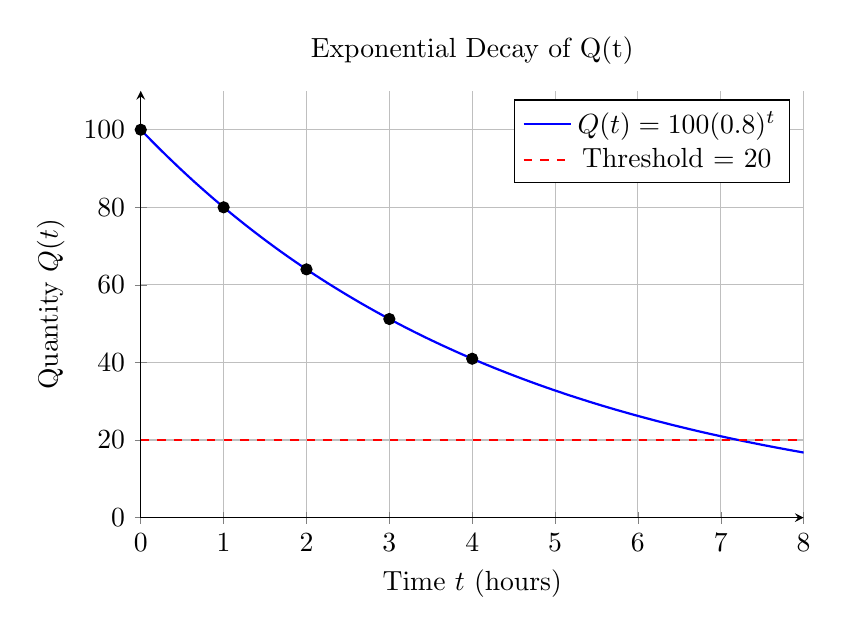
\begin{tikzpicture}
\begin{axis}[
    title={Exponential Decay of Q(t)},
    xlabel={Time $t$ (hours)},
    ylabel={Quantity $Q(t)$},
    axis lines=left,
    grid=major,
    domain=0:8,
    samples=100,
    width=10cm, height=7cm,
    ymin=0, ymax=110
]
\addplot[color=blue, thick] {100 * 0.8^x};
\addlegendentry{$Q(t) = 100(0.8)^t$}

\addplot[color=red, dashed] coordinates {(0,20) (8,20)};
\addlegendentry{Threshold = 20}

\addplot[
    color=black,
    mark=*,
    only marks
    ]
    coordinates {
    (0,100)(1,80)(2,64)(3,51.2)(4,40.96)
    };
\end{axis}
\end{tikzpicture}
\end{center}
\pagebreak

\subsection{Problem 2. Transformations, composition, and inverse}
Let
\[f(x)=\sqrt{4-(x-1)^{2}}, \quad g(x)=\ln(x+2),\]
with appropriate domains.

\begin{enumerate}[label=(\alph*)]
    \item Describe how the graph of $y=f(x)$ can be obtained from the graph of $y=\sqrt{4-x^{2}}$ using translations and/or reflections. Determine the domain and range of $f$.
    \item Determine the domain of $g$ and find the inverse function $g^{-1}$. Verify your answer by composition.
    \item Consider the composition $h(x)=f(g(x))$. Determine the domain of $h$ and explain why the domain is more restrictive than that of $g$ alone.
    \item Sketch (roughly but clearly) the graphs of $y=g(x)$ and $y=h(x)$ on the same axes. Discuss how the behavior of $h$ near the left endpoint of its domain reflects the constraints coming from $f$.
\end{enumerate}

\subsection*{Strategy}
\subsection*{Solution}
\pagebreak
\subsection{Problem 3. Trigonometric modeling}
The number of hours of daylight $D$ in a certain city can be approximated as a function of the day of the year $t$ (measured in days, with $t=0$ on January 1) by a sinusoidal model:
\[D(t)=A+B \cos(\omega(t-t_{0})).\]
Suppose you are given that the longest day has 14 hours of daylight (around day $t\approx172$) and the shortest day has 10 hours of daylight (around day $t\approx355$).

\begin{enumerate}[label=(\alph*)]
    \item Determine $A$ and $B$ from the information about the longest and shortest days. Explain the meaning of these two parameters.
    \item Argue that a reasonable choice for $\omega$ is $\dfrac{2\pi}{365}$. Explain briefly where this comes from.
    \item Choose a suitable value of $t_{0}$ so that the maximum of $D(t)$ occurs around $t=172$. Write the explicit function $D(t)$ with your chosen parameters.
    \item Using your model, estimate the number of hours of daylight on day $t=80$ and discuss qualitatively how accurate you expect the model to be (e.g., weather effects, geographical assumptions).
\end{enumerate}

\subsection*{Strategy}
\subsection*{Solution}

\pagebreak

\section{Chapter 2: Limits, Derivatives and Applications}
\subsection{Problem 4. Limits and continuity with a parameter}
Consider the functions:
\[ f(x)=\begin{cases}\dfrac{x^{2}-1}{x-1},&x\ne1,\\ a,&x=1,\end{cases} \quad \text{and} \quad g(x)=\begin{cases}\dfrac{\sin(bx)}{x},&x\ne0,\\ 1,&x=0,\end{cases} \]
where $a$ and $b$ are real parameters.

\begin{enumerate}[label=(\alph*)]
    \item Compute $\displaystyle\lim_{x\rightarrow1}\frac{x^{2}-1}{x-1}$ and $\displaystyle\lim_{x\rightarrow0}\frac{\sin(bx)}{x}$ (express your answer for the second limit in terms of $b$).
    \item Find the values of $a$ and $b$ such that $f$ is continuous at $x=1$ and $g$ is continuous at $x=0$.
    \item For your chosen values of $a$ and $b$, sketch the graphs of $f$ and $g$ near the problematic points and explain how the value at the point is "patched" to make the function continuous.
    \item Explain why changing only the value at a single point can never make a function differentiable at that point if the two one-sided derivatives from the limit expression disagree.
\end{enumerate}

\subsection*{Strategy}
\subsection*{Solution}

\pagebreak
\subsection{Problem 5. Derivative from first principles and non-differentiability}
Let
\[h(x)=\sqrt{x}, \quad x>0, \quad\quad k(x)=|x-2|.\]

\begin{enumerate}[label=(\alph*)]
    \item Using the limit definition of the derivative, compute $h^{\prime}(a)$ for an arbitrary $a>0$.
    \item Compute $k^{\prime}(x)$ using the limit definition at the point $x=2$ by considering one-sided limits. Explain why $k$ is not differentiable at $x=2$.
    \item Sketch the graphs of $y=h(x)$ and $y=k(x)$ and interpret geometrically your results about differentiability.
    \item Explain clearly the difference between continuity and differentiability by comparing the behavior of $h$ and $k$ at the points $x=0$ (for $h$) and $x=2$ (for $k$).
\end{enumerate}

\subsection*{Strategy}
\subsection*{Solution}
\pagebreak
\subsection{Problem 6. Intermediate Value Theorem and root existence}
Define
\[F(x)=x^{3}-3x+1.\]

\begin{enumerate}[label=(\alph*)]
    \item Show that $F$ is continuous on $\mathbb{R}$ and evaluate $F(0)$, $F(1)$, and $F(2)$.
    \item Use the Intermediate Value Theorem to prove that $F(x)=0$ has at least one real root in the interval $(0, 1)$.
    \item Discuss how this reasoning generalizes: how can one combine continuity and derivative information to locate and count real roots of a polynomial?
\end{enumerate}

\subsection*{Strategy}
\subsection*{Solution}
\pagebreak
\subsection{Problem 7. Differentiation rules and linear approximation}
Let
\[f(x)=\frac{e^{2x}}{x^{2}+1}.\]

\begin{enumerate}[label=(\alph*)]
    \item Compute $f^{\prime}(x)$ using the quotient rule and the chain rule. Simplify your result as much as reasonably possible.
    \item Find the linear approximation (tangent line approximation) of $f$ at $x=0$ and use it to approximate $f(0.1)$.
    \item Give a numerical estimate of the absolute error between your linear approximation and the exact value of $f(0.1)$ (you may use a calculator for the exponential).
    \item Explain why the linear approximation is expected to be accurate near $x=0$ and why it becomes less reliable as $|x|$ grows. Relate this discussion to the second derivative of $f$.
\end{enumerate}

\subsection*{Strategy}
\subsection*{Solution}
\pagebreak
\subsection{Problem 8. Related rates: moving shadow}
A lamp is mounted at the top of a 5-m high pole. A person who is 1.8 m tall walks away from the base of the pole along a straight path at a speed of $1.2\text{ m/s}$. Assume the lamp is a point source.

\begin{enumerate}[label=(\alph*)]
    \item Draw a diagram and introduce notation for the distance $x(t)$ of the person from the pole and the length $s(t)$ of the shadow on the ground.
    \item Use similar triangles to derive a relationship between $x$ and $s$.
    \item Use related rates to find $\dfrac{ds}{dt}$ when $x=10\text{ m}$. Interpret the sign and magnitude of $\dfrac{ds}{dt}$.
    \item Determine the speed of the tip of the shadow at the same moment, and compare it with the speed of the person.
\end{enumerate}

\subsection*{Strategy}
\subsection*{Solution}
\pagebreak
\subsection{Problem 9. Optimization with cost}
A box with a square base and open top must have a volume of $32\text{ m}^{3}$. The material for the base costs \$10 per square meter, and the material for the sides costs \$6 per square meter.

\begin{enumerate}[label=(\alph*)]
    \item Let $x$ be the side length of the square base (in meters) and $h$ the height. Express $h$ in terms of $x$ using the volume constraint.
    \item Write the cost $C(x)$ of materials as a function of $x$ only. Simplify your expression.
    \item Find the value of $x$ (and corresponding $h$) that minimizes the cost. Justify that your solution gives a minimum using the first or second derivative test.
\end{enumerate}

\subsection*{Strategy}
\subsection*{Solution}
\pagebreak
\subsection{Problem 10. Mean Value Theorem and inequalities}
Let $f(x)=\ln(1+x)$, defined for $x>-1$.

\begin{enumerate}[label=(\alph*)]
    \item State the Mean Value Theorem (MVT) precisely.
    \item Use the MVT to prove that for $x>-1$:
    \[ \frac{x}{1+x} \le \ln(1+x) \le x \]
    (Hint: consider $f(x)$ on a suitable interval and apply the MVT to an appropriate auxiliary function.)
    \item Interpret these inequalities graphically by sketching $y=\ln(1+x)$ together with $y=x$ and $y=\dfrac{x}{1+x}$.
    \item Explain how such inequalities can be used to estimate logarithms without a calculator and to bound errors in numerical methods.
\end{enumerate}

\subsection*{Strategy}
\subsection*{Solution}
\pagebreak

\section{Chapter 3: Integrals and Applications}
\subsection{Problem 11. Riemann sums and a parameter}
Let $f(x)=x^{2}+2x$ on the interval $[0, a]$, where $a>0$ is a constant.

\begin{enumerate}[label=(\alph*)]
    \item Construct the right-endpoint Riemann sum $R_{n}$ for $\displaystyle\int_{0}^{a}f(x)dx$ using $n$ equal subintervals. Express $R_{n}$ explicitly as a sum.
    \item Rewrite $R_{n}$ using sigma notation and known formulas for $\sum_{k=1}^{n}k$ and $\sum_{k=1}^{n}k^{2}$.
    \item Compute $\lim_{n\rightarrow\infty}R_{n}$ and verify that the result matches the antiderivative computation of $\displaystyle\int_{0}^{a}f(x)dx$.
    \item Interpret your final expression as an area and discuss how it depends on the parameter $a$. What happens if you double $a$?
\end{enumerate}

\subsection*{Strategy}
\begin{enumerate}[label = (\alph*)]
    \item To construct the right-endpoint Riemann sum $R_n$, we first construct the $n$ equal subintervals. We then calculate the area for each rectangle in the corresponding subinterval and express $R_n$ as the sum of these areas.
    \item To rewrite $R_n$, we use mathematical operations to find out the formula of $R_n$.
    \item We first compute $\lim_{n\to\infty} R_{n}$. Next, we calculate the antiderivative computation of $\int_0^af(x)dx$ and illustrate that the values computed are the same.
    \item We express the final expression geometrically and show the relationship between the area and the parameter a.
\end{enumerate}
\subsection*{Solution}

\textbf{(a) Construction and expression of $\mathbf{R_n}$}
    \begin{itemize}
    \item \textbf{Construction:} \\
    To start with, we construct the $n$ equal subintervals. Since there are $n$ equal subintervals in the interval $[0, a]$, the width of each rectangle in the corresponding subinterval is: 
    \begin{equation*}
        \Delta x = \frac{a - 0}{n} = \frac{a}{n}
    \end{equation*}
    We denote $x_i$ as the endpoint of the subintervals. The $n$ equal subintervals can be displayed as: 
    \[[x_0, x_1], [x_1, x_2],...,[x_{n-1}, x_n]\]
    \centerline {Where: \(x_i = x_0 + i\Delta x = \frac{ia}{n}\)} \\
    Since we are dealing with right-endpoint, the height of the rectangle in the subinterval $[x_{i-1}, x_i]$ is $f(x_i)$. \\
    Therefore, we achieve the area of the $i^{th}$ rectangle as: \(f(x_i)\Delta x\). \\
    \item \textbf{Expression:} \\
    Taking the sum of all of the rectangle areas gives us: 
    \begin{equation*}
    \begin{split}
        R_n &= \sum_{i=1}^n f(x_i)\Delta x \\
        &= \sum_{i=1}^n (x_i^2 + 2x_i)\frac{a}{n} \\
        &= \sum_{i=1}^n [(\frac{ia}{n})^2 + 2\frac{ia}{n}]\frac{a}{n} \\
        &= \sum_{i=1}^n (\frac{i^{2}a^{3} + 2ia^{2}n}{n^3})
    \end{split}
    \end{equation*}
    Hence,
    \begin{center} \fbox{$\displaystyle R_n = \sum_{i=1}^n (\frac{i^{2}a^{3} + 2ia^{2}n}{n^3})$} \end{center}
    \end{itemize}

\textbf{(b) Rewriting $\mathbf{R_n}$} \\
    To rewrite $R_n$, we first notice that the formula of $R_n$ contains the constant \(\displaystyle\frac{a^2}{n^2}\), which can be put outside the sigma notation.\\
    We rewrite $R_n$ as: \[R_n = \frac{a^2}{n^2}\sum_{i=1}^n (\frac{i^{2}a}{n} + 2i)\]
    Let \[S = \sum_{i=1}^n (\frac{i^{2}a}{n} + 2i)\] 
    \begin{equation}
    \Longrightarrow R_n = \frac{a^2}{n^2}\cdot S
    \end{equation}
    We calculate $S$ :
    \begin{align*}
        S &= \sum_{i=1}^n (\frac{i^{2}a}{n} + 2i) \\
        &= \frac{a}{n}\sum_{i=1}^n i^2 + 2\sum_{i=1}^ni\\
    \end{align*}
    By applying the formulas:  \[\sum_{k=1}^n k = \frac{n(n+1)}{2}\quad; \quad\sum_{k=1}^n k^2 = \frac{n(n+1)(2n+1)}{6}\], we get: \\
    \begin{align*}
        S &= \frac{a}{n} \cdot \frac{n(n+1)(2n+1)}{6} + 2\cdot \frac{n(n+1)}{2} \\
        \iff S &= \frac{a(n+1)(2n+1)}{6} + n(n+1) 
    \end{align*}
    Substituting the formula of S into (3) gives us:
    
    \begin{center} \fbox{$\displaystyle R_n = \frac{a^3 (n+1)(2n+1)}{6n^2} + \frac{a^2 (n+1)}{n}$} \end{center}

\textbf{(c) Limit computation and verification:}
    \begin{itemize} 
    \item \textbf{Limit calculation:}
    \begin{align*}
        \lim_{n\to \infty} R_n &= \lim_{n\to \infty} [\frac{a^3 (n+1)(2n+1)}{6n^2} + \frac{a^2 (n+1)}{n} ] \\
        &= \lim_{n\to \infty} [\frac{a^3 (n+1)(2n+1) + a^2 6n(n+1)}{6n^2} ] \\
        &= \lim_{n\to \infty} [\frac{(2a^3 + 6a^2)n^2 + (3a^3 + 6a^2)n + a^3}{6n^2} ] \\
        &= \lim_{n\to \infty} [\frac{(2a^3 + 6a^2) + \frac{3a^3 + 6a^2}{n} + \frac{a^3}{n^2}}{6} ] \\
        \intertext{Using the limit property $\displaystyle\lim_{n \to \infty} \frac{c}{n^k} = 0$ for $k > 0$, we get: } \\
        \lim_{n\to \infty} R_n &= \lim_{n\to \infty} [\frac{(2a^3 + 6a^2) + 0 + 0}{6} ] \\
        &= \lim_{n\to \infty} (\frac{a^3}{3} + a^2) \\
        &= \frac{a^3}{3} + a^2 
    \end{align*}
    Thus, \begin{equation}
    \lim_{n\to \infty} R_n = \frac{a^3}{3} + a^2
    \end{equation}
    \item \textbf{Antiderivative computation:}
    \begin{align*}
        \int_0^af(x)dx &= \int_0^a (x^2 + 2x)dx \\
        &= \left. \frac{x^3}{3} + x^2 \right|_{x=0}^{x=a}\\
    \end{align*}
    \begin{equation}
        \Longleftrightarrow \int_0^af(x)dx  = \frac{a^3}{3} + a^2
    \end{equation}
    \item \textbf{Verification:}
    From (4) and (5), it can be seen that the Riemann sum limit matches the antiderivative result. Hence, the computation is verified.
    \end{itemize}
    
\textbf{(d) Interpretation and Parameter Dependence:}
    The final expression $A(a) = \frac{a^3}{3} + a^2$ represents the \textbf{exact area} under the curve $f(x)=x^2+2x$ from $x=0$ to $x=a$.
    
    \begin{itemize}
        \item \textbf{Dependence on $\mathbf{a}$:} The area $A(a)$ is a polynomial function of degree 3 in terms of the parameter $a$. This confirms that the area is highly sensitive to the width of the interval.
    
        \item \textbf{Doubling $\mathbf{a}$:} If we double the width of the interval from $a$ to $2a$, the new area is $A(2a)$:
        \[
        A(2a) = \frac{(2a)^3}{3} + (2a)^2 = \frac{8a^3}{3} + 4a^2
        \]
        Since $A(2a) \neq 2 \cdot A(a)$, doubling the width of the interval more than doubles the area due to the cubic and quadratic growth terms.
    \end{itemize}
\pagebreak
\subsection{Problem 12. Fundamental Theorem of Calculus and average value}
Let
\[F(x)=\displaystyle\int_{0}^{x}\sqrt{t^{4}+2}dt, \quad x\in\mathbb{R}\]

\begin{enumerate}[label=(\alph*)]
    \item Use the Newton-Leibniz formula to compute $F^{\prime}(x)$.
    \item Find the average value of the function $f(x)=x^{3}+2x$ on the interval $[-1, 2]$.
    \item Find all points $c$ in $[-1,2]$ such that $f(c)$ equals the average value from part (b). Justify using the Mean Value Theorem for integrals.
    \item In a physical context where $f(x)$ represents a velocity, explain the meaning of the average value of $f$ on $[-1,2]$ and of the points $c$ found above.
\end{enumerate}

\subsection*{Strategy}
\subsection*{Solution}
\pagebreak
\subsection{Problem 13. Area between curves and splitting the region}
Consider the curves
\[y=x^{3}, \quad y=x, \quad y=-2\]

\begin{enumerate}[label=(\alph*)]
    \item Sketch the three curves on the same coordinate plane. Determine all intersection points relevant to the bounded region enclosed by these curves.
    \item Express the area of the shaded region (bounded by the three curves) as a sum of one or more definite integrals. Clearly justify the limits and integrands you choose.
    \item Evaluate the area exactly.
    \item Discuss how the setup would change if you integrated with respect to $y$ instead of $x$. Which method seems more natural here, and why?
\end{enumerate}

\subsection*{Strategy}
\subsection*{Solution}
\pagebreak
\subsection{Problem 14. Volumes by disks and shells}
A solid is obtained by rotating the region bounded by $y=x^{2}$, $y=0$, and $x=1$ about:
\begin{enumerate}[label=(\alph*)]
    \item The $x$-axis (use the disk/washer method).
    \item The line $x=2$ (use the shell method).
\end{enumerate}

\begin{enumerate}[label=(\alph*), start=3]
    \item Set up (but do not yet evaluate) the integral for the volume in case (a), then compute it.
    \item Set up and evaluate the integral for the volume in case (b). Simplify as much as possible.
    \item Compare the two methods (disks vs shells) in each case and explain which is more convenient and why. Would it still be the case if the region were more complicated?
\end{enumerate}

\subsection*{Strategy}
\subsection*{Solution}
\begin{center}
\begin{tikzpicture}
    \begin{axis}[
        axis lines=middle,
        xlabel=$x$, ylabel=$y$,
        xmin=-0.5, xmax=2.5,
        ymin=-0.5, ymax=1.5,
        width=0.6\textwidth,
        height=0.6\textwidth
    ]
        % Plot y = x^2
        \addplot[name path=A, blue, thick, domain=0:1] {x^2};
        
        % Plot y = 0 (x-axis)
        \addplot[name path=B, black, thick, domain=0:1] {0};
        
        % Plot x = 1
        \addplot[black, thick] coordinates {(1,0) (1,1)};

        % Shade the region
        \addplot[gray!30] fill between[of=A and B];
        \node at (axis cs:0.7, 0.2) {Region};

        % Draw Axis of Rotation for (b)
        \addplot[red, dashed, thick] coordinates {(2,-0.5) (2,1.5)};
        \node[red, right] at (axis cs:2, 0.8) {Axis $x=2$};
        
    \end{axis}
\end{tikzpicture}
\end{center}
\textbf{(c) Volume about the x-axis (Disk Method)}
Since we are rotating about the x-axis, the cross-section at $x$ is a disk with radius $R(x) = x^2$.
\[ V_a = \int_{0}^{1} \pi [R(x)]^2 dx = \pi \int_{0}^{1} (x^2)^2 dx \]
Computing the integral:
\[ V_a = \pi \int_{0}^{1} x^4 dx = \pi \left[ \frac{x^5}{5} \right]_{0}^{1} = \pi \left( \frac{1}{5} - 0 \right) = \boxed{\frac{\pi}{5}} \]

\textbf{(d) Volume about the line x=2 (Shell Method)}
We use cylindrical shells with thickness $dx$.
\begin{itemize}
    \item \textbf{Radius ($r$):} The distance from the slice at $x$ to the axis $x=2$ is $r = 2 - x$.
    \item \textbf{Height ($h$):} The height of the function at $x$ is $h = x^2$.
\end{itemize}
The volume formula is $V = \int_{a}^{b} 2\pi r h \, dx$.
\[ V_b = \int_{0}^{1} 2\pi (2-x)(x^2) dx \]
Evaluating the integral:
\[ V_b = 2\pi \int_{0}^{1} (2x^2 - x^3) dx \]
\[ V_b = 2\pi \left[ \frac{2x^3}{3} - \frac{x^4}{4} \right]_{0}^{1} \]
\[ V_b = 2\pi \left( \left(\frac{2}{3} - \frac{1}{4}\right) - 0 \right) = 2\pi \left( \frac{8-3}{12} \right) = 2\pi \left(\frac{5}{12}\right) = \boxed{\frac{5\pi}{6}} \]

\textbf{(e) Comparison of Methods}
\begin{itemize}
    \item \textbf{Case (a):} The Disk method was very convenient because the rotation axis ($y=0$) was a boundary of the region, and the function $y=x^2$ was explicitly given. Using shells here would require integrating with respect to $y$ (horizontal shells), involving $x=\sqrt{y}$, which is slightly more complex.
    \item \textbf{Case (b):} The Shell method was convenient because we could continue using the variable $x$. If we used the Washer method (slices perpendicular to $x=2$, i.e., horizontal $dy$), we would need:
    \begin{itemize}
        \item Outer radius $R_{out} = 2 - 0 = 2$ (distance from axis to y-axis).
        \item Inner radius $R_{in} = 2 - \sqrt{y}$ (distance from axis to curve).
    \end{itemize}
    The integral would be $\pi \int_0^1 (2^2 - (2-\sqrt{y})^2) dy$, which involves more algebra to expand.
    \item \textbf{Conclusion:} The shell method is generally better when rotating about vertical lines for functions given as $y=f(x)$, as it avoids solving for $x$ and dealing with potentially complicated inverse functions.
\end{itemize}
\pagebreak

\subsection{Problem 15. Substitution with definite integrals}
Evaluate the following definite integrals using appropriate substitutions:
\[I_{1}=\int_{0}^{1}\frac{2x}{1+x^{2}}dx, \quad I_{2}=\int_{0}^{\pi/2}\sin^{3}x \cos x dx, \quad I_{3}=\int_{1}^{e}\frac{\ln x}{x}dx.\]

\begin{enumerate}[label=(\alph*)]
    \item Evaluate $I_{1}$ and explain why a substitution of the form $u=1+x^{2}$ is natural.
    \item Evaluate $I_{2}$ and explain your choice of substitution in terms of recognizing a derivative inside the integrand.
    \item Evaluate $I_{3}$ and then differentiate your result with respect to the upper limit $e$ to check consistency with the FTC.
    \item For one of the integrals above, propose an incorrect substitution and explain why it fails or complicates the problem, illustrating the importance of a good choice.
\end{enumerate}

\subsection*{Strategy}
To evaluate these definite integrals, we look for a substitution $u = g(x)$ such that the derivative $g'(x)dx$ (or a multiple of it) appears in the integrand. The general strategy is:
\begin{enumerate}[label = (\alph*)]
    \item \textbf{Identify the inner function:} Look for a function "inside" another function (e.g., inside a denominator, a power, or a logarithm).
    \item \textbf{Check the derivative:} Verify if the derivative of that inner function is present as a multiplicative factor.
    \item \textbf{Change limits}
\end{enumerate}

\subsection*{Solution}
\textbf{(a) Evaluation of $I_1$:} \\
    We have $I_1 = \int_{0}^{1} \frac{2x}{1+x^2} dx$.
    \begin{itemize}
        \item Let $u = 1 + x^2$. Then, $du = 2x \, dx$.
        \item
        \begin{itemize}
            \item When $x = 0 \implies u = 1 + 0^2 = 1$.
            \item When $x = 1 \implies u = 1 + 1^2 = 2$.
        \end{itemize} 
        \item \textbf{We have:}
        \[
        I_1 = \int_{1}^{2} \frac{1}{u} \, du = \ln|u| \Big|_{1}^{2} = \ln(2) - \ln(1) = \ln(2).
        \]
        \item \textbf{Explanation:} The substitution $u = 1 + x^2$ is natural because the numerator $2x$ is exactly the derivative of the denominator $1 + x^2$. This transforms a rational function into a standard natural logarithm integral form $\int \frac{du}{u}$.
    \end{itemize}

\textbf{(b) Evaluation of $I_2$:} \\
    We have $I_2 = \int_{0}^{\pi/2} \sin^3 x \cos x \, dx$.
    \begin{itemize}
        \item Let $u = \sin x$. Then, $du = \cos x \, dx$.
        \item
        \begin{itemize}
            \item When $x = 0 \implies u = \sin(0) = 0$.
            \item When $x = \pi/2 \implies u = \sin(\pi/2) = 1$.
        \end{itemize}
        \item \textbf{We have:}
        \[
        I_2 = \int_{0}^{1} u^3 \, du = \frac{u^4}{4} \Big|_{0}^{1} = \frac{1^4}{4} - \frac{0^4}{4} = \frac{1}{4}.
        \]
        \item \textbf{Explanation:} We recognize that $\cos x$ is the derivative of $\sin x$. Since $\sin x$ is raised to a power, choosing $u = \sin x$ absorbs the $\cos x$ term into $du$, simplifying the integrand to a basic power rule form $u^n$.
    \end{itemize}

\textbf{(c) Evaluation of $I_3$ and FTC Check:} \\
    We have $I_3 = \int_{1}^{e} \frac{\ln x}{x} dx = \int_{1}^{e} (\ln x) \cdot \frac{1}{x} dx$.
    \begin{itemize}
        \item Let $u = \ln x$. Then, $du = \frac{1}{x} dx$.
        \item
        \begin{itemize}
            \item When $x = 1 \implies u = \ln(1) = 0$.
            \item When $x = e \implies u = \ln(e) = 1$.
        \end{itemize}
        \item \textbf{We have:}
        \[
        I_3 = \int_{0}^{1} u \, du = \frac{u^2}{2} \Big|_{0}^{1} = \frac{1}{2} - 0 = \frac{1}{2}.
        \]
        \item \textbf{FTC Check:} Consider the integral with a variable upper limit $t$: $A(t) = \int_{1}^{t} \frac{\ln x}{x} dx = \frac{(\ln t)^2}{2}$.
        Differentiating this result with respect to $t$:
        \[
        A'(t) = \frac{1}{2} \cdot 2(\ln t) \cdot (\ln t)' = (\ln t) \cdot \frac{1}{t} = \frac{\ln t}{t}.
        \]
        This matches the original integrand.
    \end{itemize}

\textbf{(d) Incorrect Substitution Example:} \\
    Consider $I_1 = \int_{0}^{1} \frac{2x}{1+x^2} dx$.
    \begin{itemize}
        \item \textbf{Proposed Substitution:} Let $u = 2x$. Then $x = u/2$ and $dx = du/2$.
        \item \textbf{Resulting Integral:}
        \[
        \int \frac{u}{1 + (u/2)^2} \frac{du}{2} = \int \frac{u}{2(1 + u^2/4)} du = \int \frac{2u}{4 + u^2} du.
        \]
        \item \textbf{Why it fails/complicates:} While not mathematically "wrong" (it is still solvable), this substitution does not simplify the structure of the problem. 
    \end{itemize}
\pagebreak
\subsection{Problem 16. Integration by parts and a reduction formula}
Consider the integral
\[I_{n}=\displaystyle\int x^{n}e^{x}dx, \quad n\in\mathbb{N}\]

\begin{enumerate}[label=(\alph*)]
    \item Use integration by parts to derive a reduction formula expressing $I_{n}$ in terms of $I_{n-1}$.
    \item Use your formula to compute $I_{2}$ explicitly and check your result by direct integration.
    \item Use the reduction formula to write down $I_{3}$ (you do not need to fully expand the polynomial if it becomes too long, but express it in terms of $e^{x}$ and powers of $x$).
    \item Discuss how such a reduction formula is useful in practice, for example in symbolic computation systems or when computing moments in probability and statistics.
\end{enumerate}

\subsection*{Strategy}
To derive the reduction formula, we will evaluate the general integral for $I_n$ and express it in terms of $I_{n-1}$. Specifically, we will:

\begin{itemize}
    \item Use the integration by parts method.
    \item Derive the reduction formula.
    \item Verify the result using direct integration.
\end{itemize}
\subsection*{Solution}
\textbf{a)} 
\noindent  When $n=0$,
\[
    I_0 = \int e^x \, dx = e^x + C
\]
\noindent With $n > 0$ ,
\quad We consider the integral $I_n = \int x^n e^x \, dx$.

\noindent Using integration by parts, let us define:
\begin{align*}
    u &= x^n & \implies \quad du &= n x^{n-1} \, dx \\
    dv &= e^x \, dx & \implies \quad v &= e^x
\end{align*}

\noindent Substituting these into the formula $\int u \, dv = uv - \int v \, du$, we get:
\begin{align*}
    I_n &= x^n e^x - \int e^x \left( n x^{n-1} \right) \, dx \\
        &= x^n e^x - n \int x^{n-1} e^x \, dx \\
        &= x^n e^x - n I_{n-1}
\end{align*}

\noindent So we can conclude the reduction formula:
\[
\begin{cases}
    I_0 = e^x + C \\
    I_n = x^n e^x - n I_{n-1} \quad (\text{for } n \ge 1)
\end{cases}
\]

\vspace{1em}

\textbf{b)}

\noindent \textbf{+) Using above reduction formula:} \\
First, we compute $I_1$:
\begin{align*}
    I_1 &= x \cdot e^x - I_0 \\
        &= x \cdot e^x - e^x
\end{align*}
So, for $I_2$:
\begin{align*}
    I_2 &= x^2 \cdot e^x - 2 \cdot I_1 \\
        &= x^2 \cdot e^x - 2(x e^x - e^x) + C \\
        &= x^2 e^x - 2x e^x + 2e^x + C \quad (1)
\end{align*}

\vspace{1em}

\noindent \textbf{+) Direct integration:} \\
We have $I_2 = \int x^2 e^x \, dx$.

\noindent Let us define (1st iteration):
\begin{align*}
    u_1 &= x^2 \implies du_1 = 2x \, dx \\
    dv_1 &= e^x \, dx \implies v_1 = e^x
\end{align*}
\[ \implies I_2 = x^2 e^x - \int 2x \cdot e^x \, dx \]

\noindent Let us define (2nd iteration):
\begin{align*}
    u_2 &= 2x \implies du_2 = 2 \, dx \\
    dv_2 &= e^x \, dx \implies v_2 = e^x
\end{align*}
Substituting back:
\begin{align*}
    \implies I_2 &= x^2 e^x - \left( 2x \cdot e^x - \int 2 \cdot e^x \, dx \right) \\
    &= x^2 e^x - 2x e^x + 2 e^x + C' \quad (2)
\end{align*}

\noindent \textbf{Conclusion:} From (1) and (2), the results from the formula and direct integration are the same.
\textbf{c)} \quad Using reduction formula for $I_3$:
\begin{align*}
    I_3 &= \int x^3 e^x \, dx \\
        &= x^3 \cdot e^x - 3 \cdot I_2 \\
        &= x^3 \cdot e^x - 3 \left( x^2 e^x - 2x e^x + 2e^x + 2C \right) \\
        &= x^3 \cdot e^x - 3x^2 e^x + 6x e^x - 6e^x - 6C \\
        &= e^x \left( x^3 - 3x^2 + 6x - 6 \right) - 6C
\end{align*}
\textbf{d)} \quad \textbf{Discussion on practical usefulness:}

Such a reduction formula is highly valuable in practice for several reasons:

\begin{itemize}
    \item \textbf{Symbolic Computation Systems:}
    Computer algebra systems (like WolframAlpha, Maple, or Mathematica) rely on systematic algorithms rather than human intuition. A reduction formula transforms a complex integration problem (requiring calculus) into a sequence of simple algebraic operations (multiplication and subtraction). This allows computers to calculate the integral for any large $n$ efficiently using a recursive loop or stack, reducing the problem step-by-step to the known base case $I_0$.

    \item \textbf{Computing Moments in Probability:}
    In statistics, finding the $n$-th moment $E[X^n]$ involves integrals of the form $\int x^n f(x) \, dx$. For distributions involving exponential terms (such as the Exponential or Gamma distributions), these integrals match the form of $I_n$. The reduction formula allows us to compute higher-order moments (needed for variance, skewness, and kurtosis) sequentially from lower-order ones without performing integration by parts repeatedly for each moment.
\end{itemize}
\pagebreak
\subsection{Problem 17. Numerical integration: Trapezoidal and Simpson's Rules}
Let $f(x)=\sqrt{1+x^{3}}$ on the interval $[0, 2]$.

\begin{enumerate}[label=(\alph*)]
    \item Explain why there is no simple elementary antiderivative for $f(x)$.
    \item Approximate $\displaystyle\int_{0}^{2}f(x)dx$ using the Trapezoidal Rule with $n=4$ subintervals. Show your computations.
    \item Approximate the same integral using Simpson's Rule with $n=4$ subintervals and compare the two results.
    \item Discuss, based on the shape of the graph of $f$, which method you expect to be more accurate and why. How would you improve the accuracy further?
\end{enumerate}

\subsection*{Strategy}
\subsection*{Solution}
\pagebreak
\subsection{Problem 18. Improper integrals and comparison}
Consider the improper integral
\[J(p)=\displaystyle\int_{1}^{\infty}\frac{1}{x^{p}}dx, \quad p>0\]

\begin{enumerate}[label=(\alph*)]
    \item Evaluate $J(p)$ explicitly for all $p>1$, and show that it diverges for $0<p\le1$.
    \item Now consider the integral $\displaystyle\int_{1}^{\infty}\frac{\ln x}{x^{p}}dx$. Using comparison or limit comparison, determine for which values of $p$ this integral converges.
    \item For a specific value of $p$ where convergence holds (for example $p=3$), compute the integral $\displaystyle\int_{1}^{\infty}\frac{\ln x}{x^{3}}dx$ explicitly using integration by parts.
    \item Explain how these examples illustrate the idea that a slowly growing factor like $\ln x$ can still be dominated by a sufficiently fast decaying power $x^{-p}$.
\end{enumerate}

\subsection*{Strategy}
\subsection*{Solution}
\pagebreak
\subsection{Problem 19. Application: work done by a variable force}
A variable force (in newtons) required to stretch a spring $x$ meters beyond its natural length is given by
\[F(x)=kx+\alpha x^{2},\]
where $k>0$ and $\alpha>0$ are constants.

\begin{enumerate}[label=(\alph*)]
    \item Using Hooke's law as motivation, explain briefly why a linear term $kx$ appears, and how the additional quadratic term $\alpha x^{2}$ can model nonlinear behavior.
    \item Derive a formula for the work $W$ required to stretch the spring from $x=0$ to $x=a$ meters.
    \item Evaluate $W$ explicitly in terms of $k$, $\alpha$, and $a$.
    \item Suppose $k=40\text{ N/m}$, $\alpha=10\text{ N/m}^{2}$ and $a=0.2\text{ m}$. Compute the numerical value of the work (in joules) and discuss how much extra work is due to the nonlinear term.
\end{enumerate}

\subsection*{Strategy}
\subsection*{Solution}
\pagebreak
\subsection{Problem 20. Probability density and expectation}
Let
\[f(x)=Cxe^{-x^{2}/2}, \quad x\ge0,\]
and $f(x)=0$ for $x<0$. Assume $f$ is the probability density function of a nonnegative random variable $X$.

\begin{enumerate}[label=(\alph*)]
    \item Determine the constant $C$ so that $\displaystyle\int_{0}^{\infty}f(x)dx=1$. (Hint: use a substitution related to the Gaussian integral.)
    \item Compute the expected value $E[X]=\displaystyle\int_{0}^{\infty}xf(x)dx$.
    \item Compute the probability $P(X>1)$ and express your result in terms of the exponential function.
    \item Discuss how the tail behavior of $f(x)$ (for large $x$) affects the convergence of the integrals that define total probability and expected value.
\end{enumerate}

\subsection*{Strategy}
\subsection*{Solution}
\pagebreak

% \input{content/cite}

% References
 \input{ref/ref.tex}

 % Appendix
\appendix
 % Add \cleardoublepage to move appendices to next page.
\section{Proof of the Limit $\displaystyle \lim_{\theta \to 0} \frac{\sin \theta}{\theta} = 1$}
\label{appendix:lim}
\begin{theorem}
\[ \lim_{\theta \to 0} \frac{\sin \theta}{\theta} = 1 \]
\end{theorem}

\begin{proof}
Assume first that $\theta$ lies between $0$ and $\pi/2$. Figure 1 shows a sector of a circle with center $O$, central angle $\theta$, and radius $1$. $BC$ is drawn perpendicular to $OA$. By the definition of radian measure, we have arc $AB = \theta$. Also $|BC| = |OB|\sin\theta = \sin\theta$. From the diagram we see that
\[ |BC| < |AB| < \text{arc } AB \]

\begin{center}
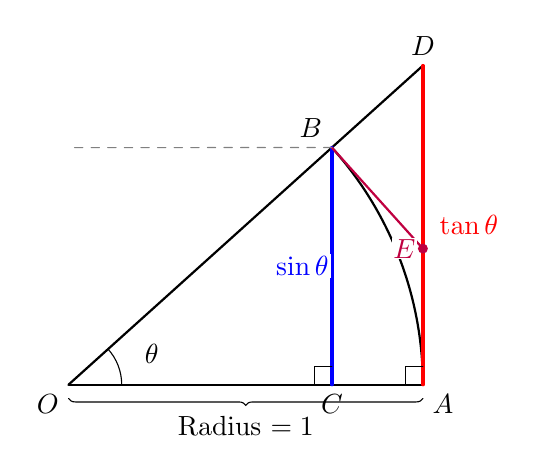
\begin{tikzpicture}[scale=4.5, cap=round, >=latex]
    % --- Definitions ---
    \def\angle{42} % Angle theta (Large enough to see clearly)
    \coordinate (O) at (0,0);
    \coordinate (A) at (1,0);
    \coordinate (B) at (\angle:1); 
    \coordinate (C) at ({cos(\angle)},0); 
    \coordinate (D) at (1,{tan(\angle)}); 
    
    % E is intersection of tangents
    % y_E = tan(theta/2)
    \coordinate (E) at (1, {(1-cos(\angle))/sin(\angle)}); 

    % --- Geometry Drawing ---
    
    % 1. The Main Sectors/Lines
    \draw[thick] (O) -- (D); % Radius extended to D
    \draw[thick] (O) -- (A); % Radius OA
    \draw[thick] (1,0) arc (0:\angle:1); % Arc AB
    
    % 2. Vertical Lines
    \draw[very thick, red] (A) -- (D); % Tangent AD
    \draw[very thick, blue] (B) -- (C); % Sine BC
    
    % 3. Tangent Segment BE
    \draw[thick, purple] (B) -- (E); 

    % 4. Dashed Projection for clarity (Optional but helps depth)
    \draw[dashed, gray] (B) -- (0, {sin(\angle)}); 

    % --- Labels with White Backgrounds to prevent overlap ---
    
    % Dimensions
    \node[red, right] at (1.02, {tan(\angle)/2}) {$\tan \theta$};
    \node[blue, left, fill=white, inner sep=1pt] at ({cos(\angle)}, {sin(\angle)/2}) {$\sin \theta$};
    
    % Points
    \node[below left] at (O) {$O$};
    \node[below] at (C) {$C$};
    \node[below right] at (A) {$A$};
    \node[above left] at (B) {$B$};
    \node[above] at (D) {$D$};
    
    % Point E (Shifted to avoid purple line)
    \fill[purple] (E) circle (0.4pt); 
    \node[left, purple, fill=white, inner sep=0.5pt, xshift=-2pt] at (E) {$E$};

    % Angle Theta
    \draw (0.15,0) arc (0:\angle:0.15);
    \node at (20:0.25) {$\theta$};
    
    % Right Angle Markers
    \draw[thin] (C) ++(-0.05,0) -- ++(0,0.05) -- ++(0.05,0); 
    \draw[thin] (A) ++(-0.05,0) -- ++(0,0.05) -- ++(0.05,0); 

    % Radius Label
    \draw[decoration={brace,mirror,raise=5pt},decorate] (O) -- (A) node[midway,below=8pt] {Radius $= 1$};
\end{tikzpicture}
\end{center}

Therefore,
\[ \sin \theta < \theta \quad \text{so} \quad \frac{\sin \theta}{\theta} < 1 \]

Let the tangent lines at $A$ and $B$ intersect at $E$. You can see from the figure that the circumference of a circle is smaller than the length of a circumscribed polygon, and so arc $AB < |AE| + |EB|$. Thus
\begin{align*}
    \theta = \text{arc } AB &< |AE| + |EB| \\
    &< |AE| + |ED| \\
    &= |AD| = |OA| \tan \theta \\
    &= \tan \theta
\end{align*}

Therefore we have
\[ \theta < \frac{\sin \theta}{\cos \theta} \]
\[ \cos \theta < \frac{\sin \theta}{\theta} < 1 \]

We know that $\lim_{\theta \to 0} 1 = 1$ and $\lim_{\theta \to 0} \cos \theta = 1$, so by the Squeeze Theorem, we have
\[ \lim_{\theta \to 0^+} \frac{\sin \theta}{\theta} = 1 \]

But the function $\dfrac{\sin \theta}{\theta}$ is an even function, so its right and left limits must be equal. Hence, we have
\[ \lim_{\theta \to 0} \frac{\sin \theta}{\theta} = 1 \]
\end{proof}
\pagebreak
\section{Proof of Chebyshev's Theorem}
\label{appendix:Chebyshev}

\begin{theorem}[Chebyshev's Theorem]
The integral of a binomial differential
\[ I = \int x^m (a + bx^n)^p \, dx, \quad \text{where } m, n, p \in \mathbb{Q} \setminus \{0\} \]
is elementary if and only if at least one of the following expressions is an integer:
\begin{enumerate}[label=(\arabic*)]
    \item $p$
    \item $\dfrac{m+1}{n}$
    \item $p + \dfrac{m+1}{n}$
\end{enumerate}
\end{theorem}

\begin{proof}
\textbf{Part 1: Sufficiency}

If one of the conditions above is met, we can transform the integral into a rational function using a specific substitution.

\begin{description}
    \item[Case (1): $p \in \mathbb{Z}$] 
    Let $k$ be the least common multiple of the denominators of $m$ and $n$. We write $m = \frac{m'}{k}$ and $n = \frac{n'}{k}$ where $k \in \mathbb{Z}^+$.
    
    Substituting $x = z^k$, we have $dx = k z^{k-1} \, dz$. The integral becomes:
    \[ 
    I = \int z^{m'} (a + b z^{n'})^p \cdot k z^{k-1} \, dz = k \int z^{m' + k - 1} (a + b z^{n'})^p \, dz 
    \]
    Since $m', n', p, k \in \mathbb{Z}$, the integrand is a rational function of $z$. Thus, $I$ is elementary.

    \item[Case (2): $\dfrac{m+1}{n} \in \mathbb{Z}$]
    Let $p = \frac{r}{t}$ where $r, t \in \mathbb{Z}$. Let $s = \dfrac{m+1}{n} \in \mathbb{Z}$.
    
    We use the substitution $u = a + bx^n$, which implies $x = \left(\frac{u-a}{b}\right)^{\frac{1}{n}}$. To eliminate the radical in $(a+bx^n)^p$, we set $u = z^t$, so $a + bx^n = z^t$.
    \[
    x = \left(\frac{z^t - a}{b}\right)^{\frac{1}{n}} \implies dx = \frac{1}{n} \left(\frac{z^t - a}{b}\right)^{\frac{1}{n} - 1} \cdot \frac{t z^{t-1}}{b} \, dz
    \]
    Substituting these into the integral:
    \[
    \begin{aligned}
    I &= \int \left(\frac{z^t - a}{b}\right)^{\frac{m}{n}} (z^t)^p \cdot \frac{t z^{t-1}}{bn} \left(\frac{z^t - a}{b}\right)^{\frac{1}{n} - 1} \, dz \\
      &= \frac{t}{bn} \int z^{r + t - 1} \left(\frac{z^t - a}{b}\right)^{\frac{m+1}{n} - 1} \, dz \\
      &= \frac{t}{bn} \int z^{r + t - 1} \left(\frac{z^t - a}{b}\right)^{s - 1} \, dz
    \end{aligned}
    \]
    Since $s, r, t \in \mathbb{Z}$, the integrand is rational in $z$. Thus, $I$ is elementary.

    \item[Case (3): $\dfrac{m+1}{n} + p \in \mathbb{Z}$]
    We rewrite the integral by factoring out $x^{np}$:
    \[ 
    I = \int x^m \cdot x^{np} (a x^{-n} + b)^p \, dx = \int x^{m+np} (b + a x^{-n})^p \, dx 
    \]
    Let $M = m+np$ and $N = -n$. Checking the condition for Case (2) on this new form:
    \[
    \frac{M+1}{N} = \frac{m+np+1}{-n} = -\left(\frac{m+1}{n} + p\right)
    \]
    Since $\frac{m+1}{n} + p \in \mathbb{Z}$, the expression $\frac{M+1}{N}$ is an integer. This reduces the problem to Case (2). Thus, $I$ is elementary.
\end{description}

\vspace{1em}
\noindent \textbf{Part 2: Remark on Necessity}

If none of the three conditions are met, the integral cannot be expressed in elementary terms. 
\begin{itemize}
    \item If $p \notin \mathbb{Z}$, the term $(a+bx^n)^p$ is a radical. To rationalize it, we must substitute $a+bx^n = z^t$. As shown in Case (2), this only yields a rational integrand if $\frac{m+1}{n} \in \mathbb{Z}$.
    \item If we attempt Integration by Parts with $u = (a+bx^n)^p$ and $dv = x^m dx$, we obtain:
    \[
    I = \frac{x^{m+1}}{m+1}(a+bx^n)^p - \frac{bpn}{m+1} \int x^{m+n}(a+bx^n)^{p-1} \, dx \quad (m \neq -1)
    \]
    The new integral requires the condition $(p-1) + \frac{m+n+1}{n} \in \mathbb{Z}$, which simplifies to $p + \frac{m+1}{n} \in \mathbb{Z}$. This does not generate a new condition but rather cycles back to the original ones.
    \item If $m = -1$ or $p = -1$, logarithmic terms appear, which prevents the integral from being algebraic unless the integer conditions are satisfied.
\end{itemize}
Therefore, the conditions are both sufficient and necessary.
\end{proof}
\end{document}